\chapter{Results}\label{chapter:results}

\section{Generation Process}

Section \ref{generate} presented two algorithms used to randomly generate tangrams. Additionally, there exist two parameters that can be adjusted to influence the generation process. The first parameter is a threshold setting the largest possible difference in x- and y-coordinates between two points. This parameter is used in both approaches. The second parameter applies only to the approach that steers towards a larger number of edge-matchings. It determines how high the probability for choosing an orientation with matched edges is compared to any other orientation. Figure \ref{eval1} shows exemplementry results of generating six tangrams for both approaches and different parameter settings. Tangrams generated by the naive approach with a range of 50 are often only connected at points and contain next to no matched edges. When reducing the threshold to 30, more matched edges exist, but the resulting shapes are also somewhat similar and square-like. However, generating only these 6 tangrams took more then 70 attempts. The edge-matching approach obviously contains more matched edges. When adjusting the probability parameter, one can see a definite effect on the result when choosing a lower value, however increasing it past the standard value of 50 has no visually obvious implementations. The effect will possibly become completely obsolete once a larger number of tangrams is generated. 

\begin{figure}[htp]
  \centering
  \subfloat[Naive approach]{\label{figur:1}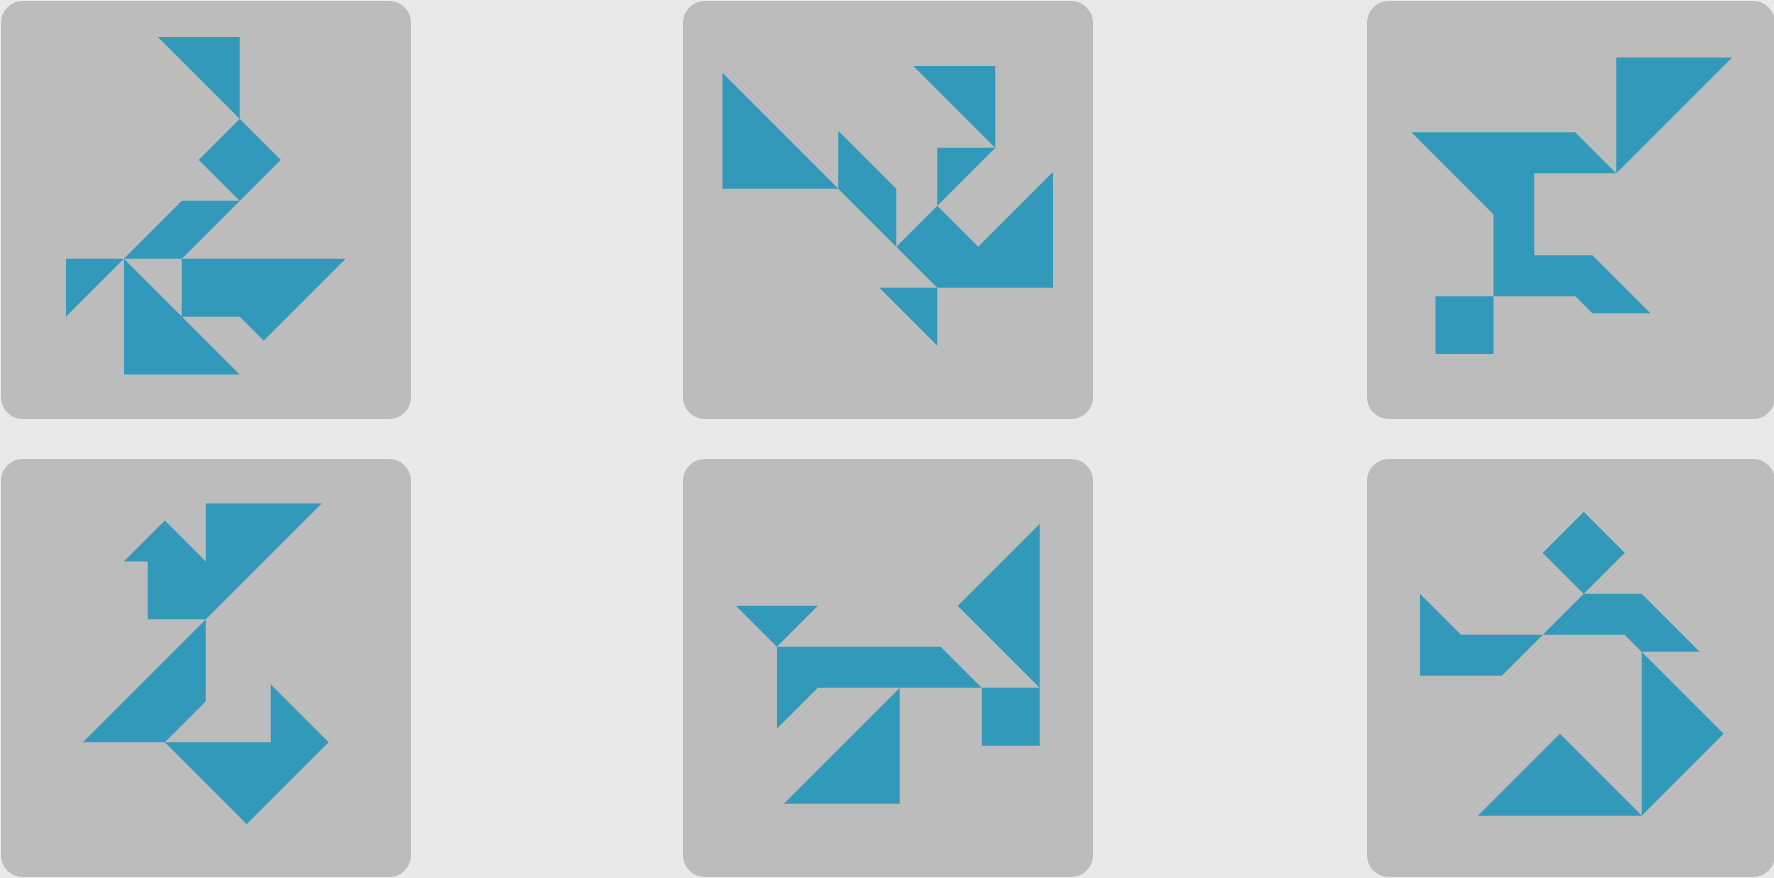
\includegraphics[width=0.45\textwidth]{figures/gen.png}}
  \hfill
  \subfloat[Naive approach with lower range threshold]{\label{figur:2}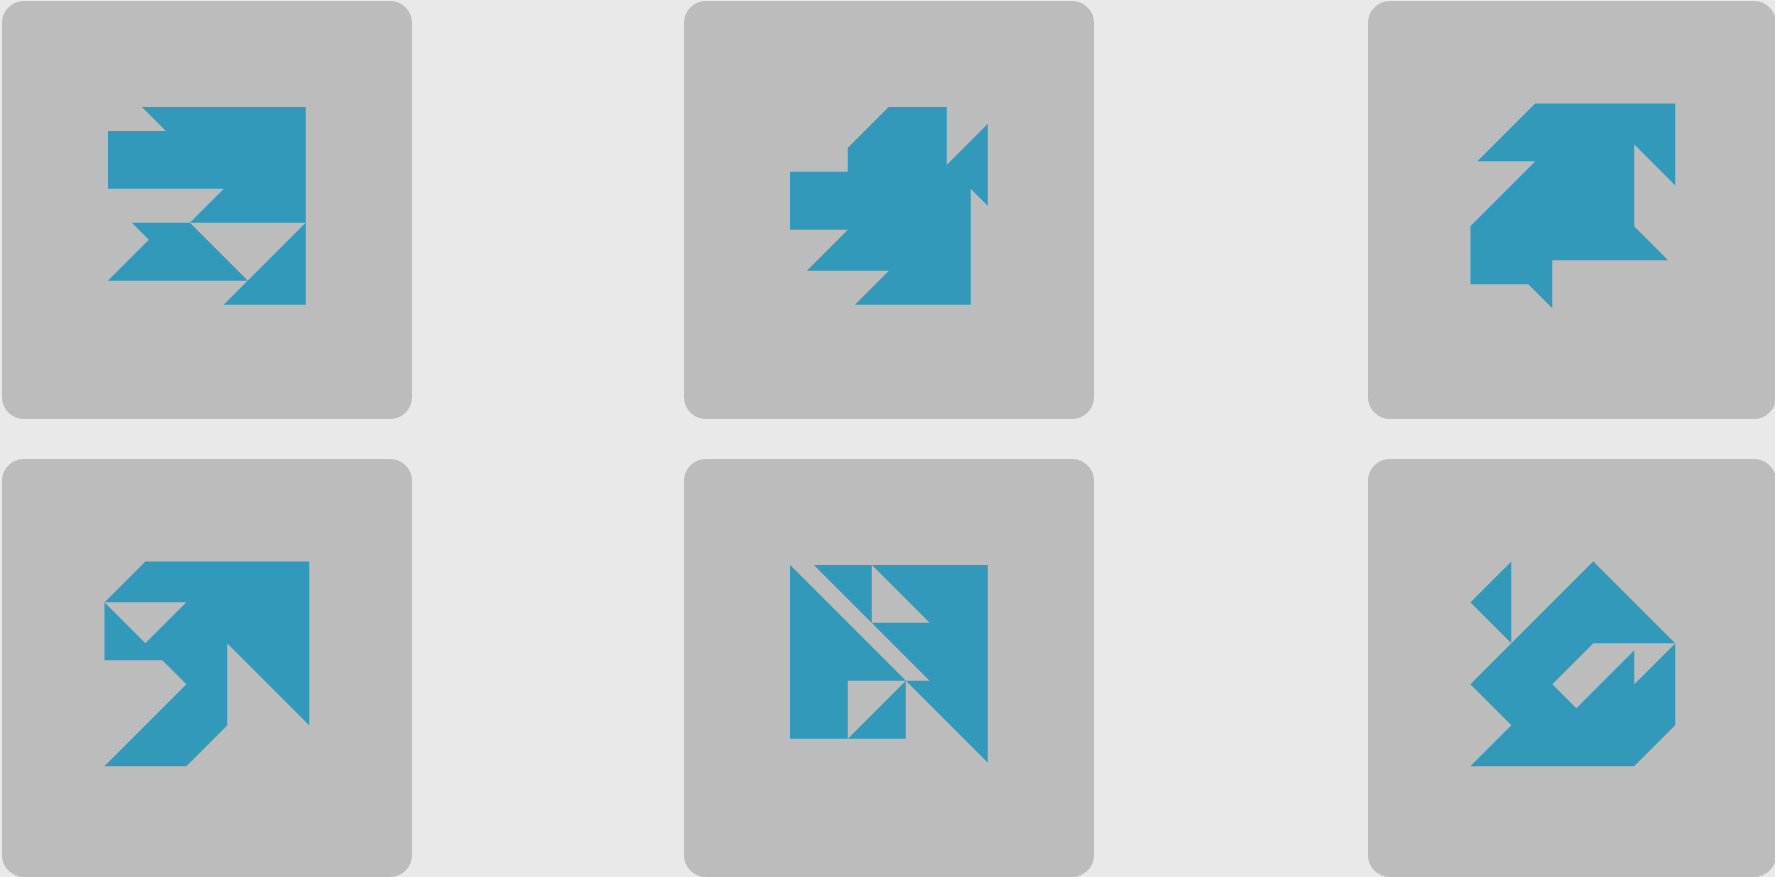
\includegraphics[width=0.45\textwidth]{figures/genSR.png}}
  \\
  \subfloat[Edge-matching approach]{\label{figur:3}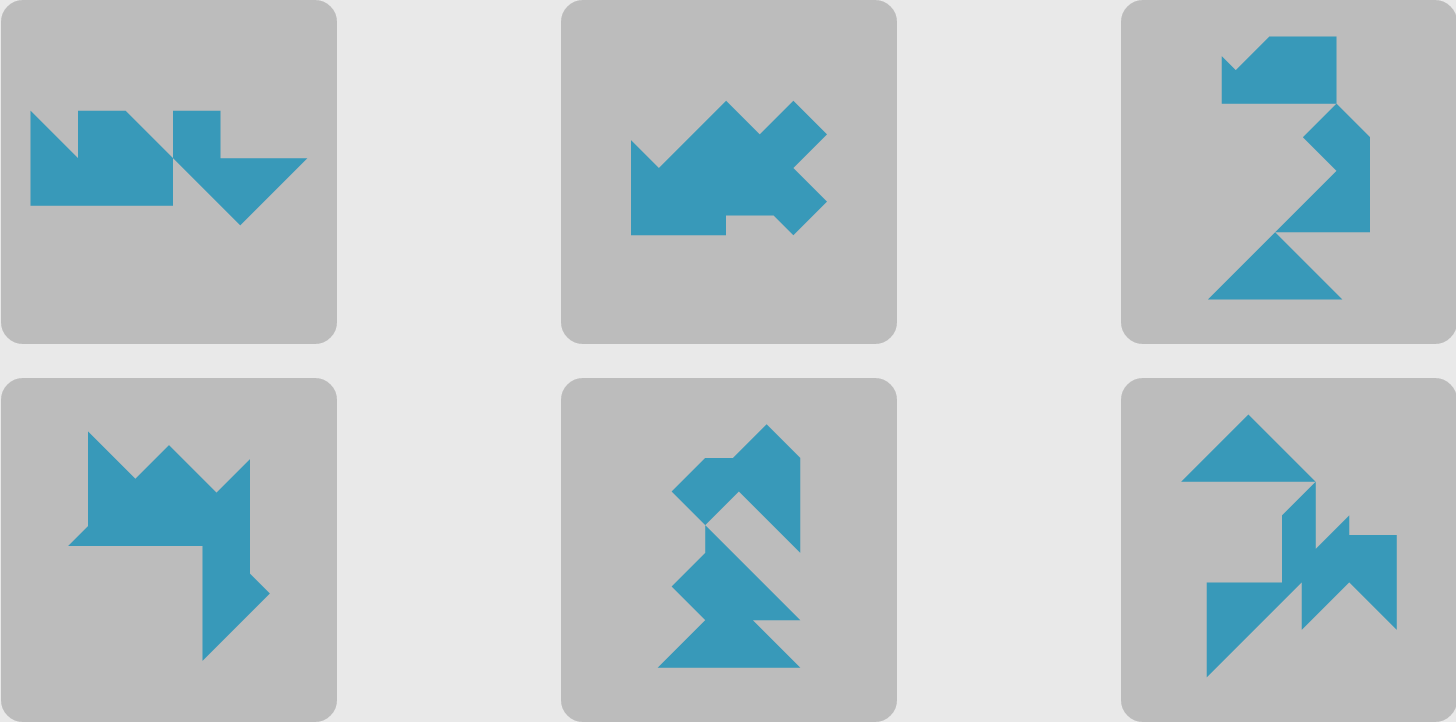
\includegraphics[width=0.45\textwidth]{figures/edges.png}}
    \hfill
  \subfloat[Edge-matching approach with lower range threshold]{\label{figur:4}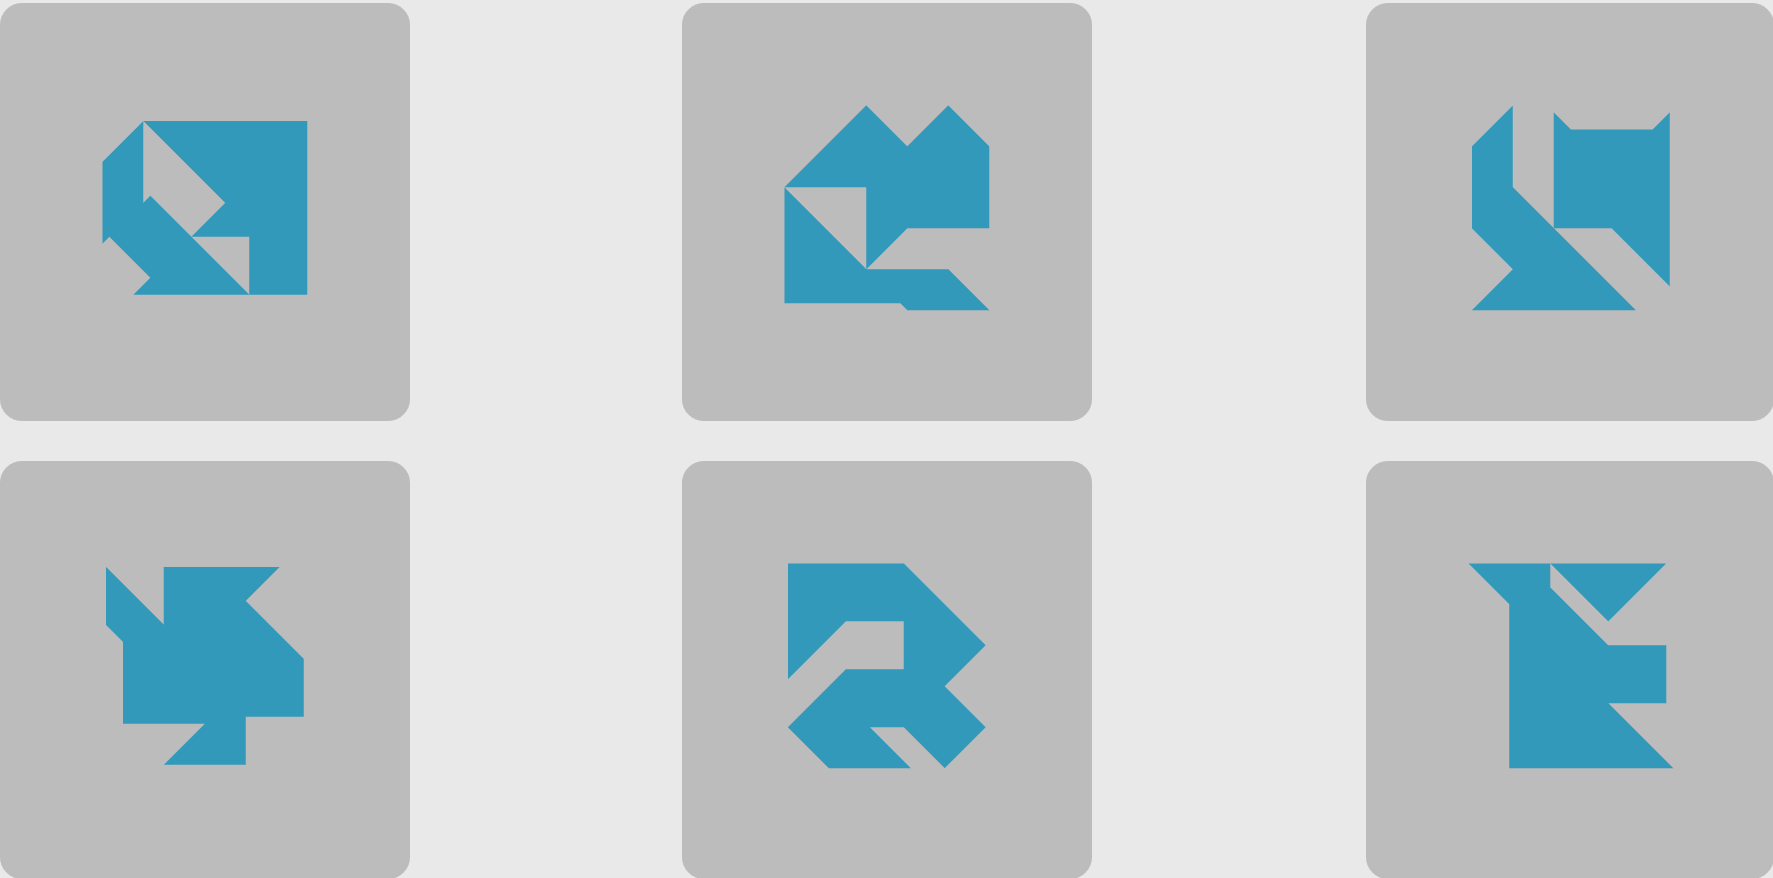
\includegraphics[width=0.45\textwidth]{figures/edgesSR.png}}
  \\
  \subfloat[Edge-matching approach with higher edge-matching weight]{\label{figur:5}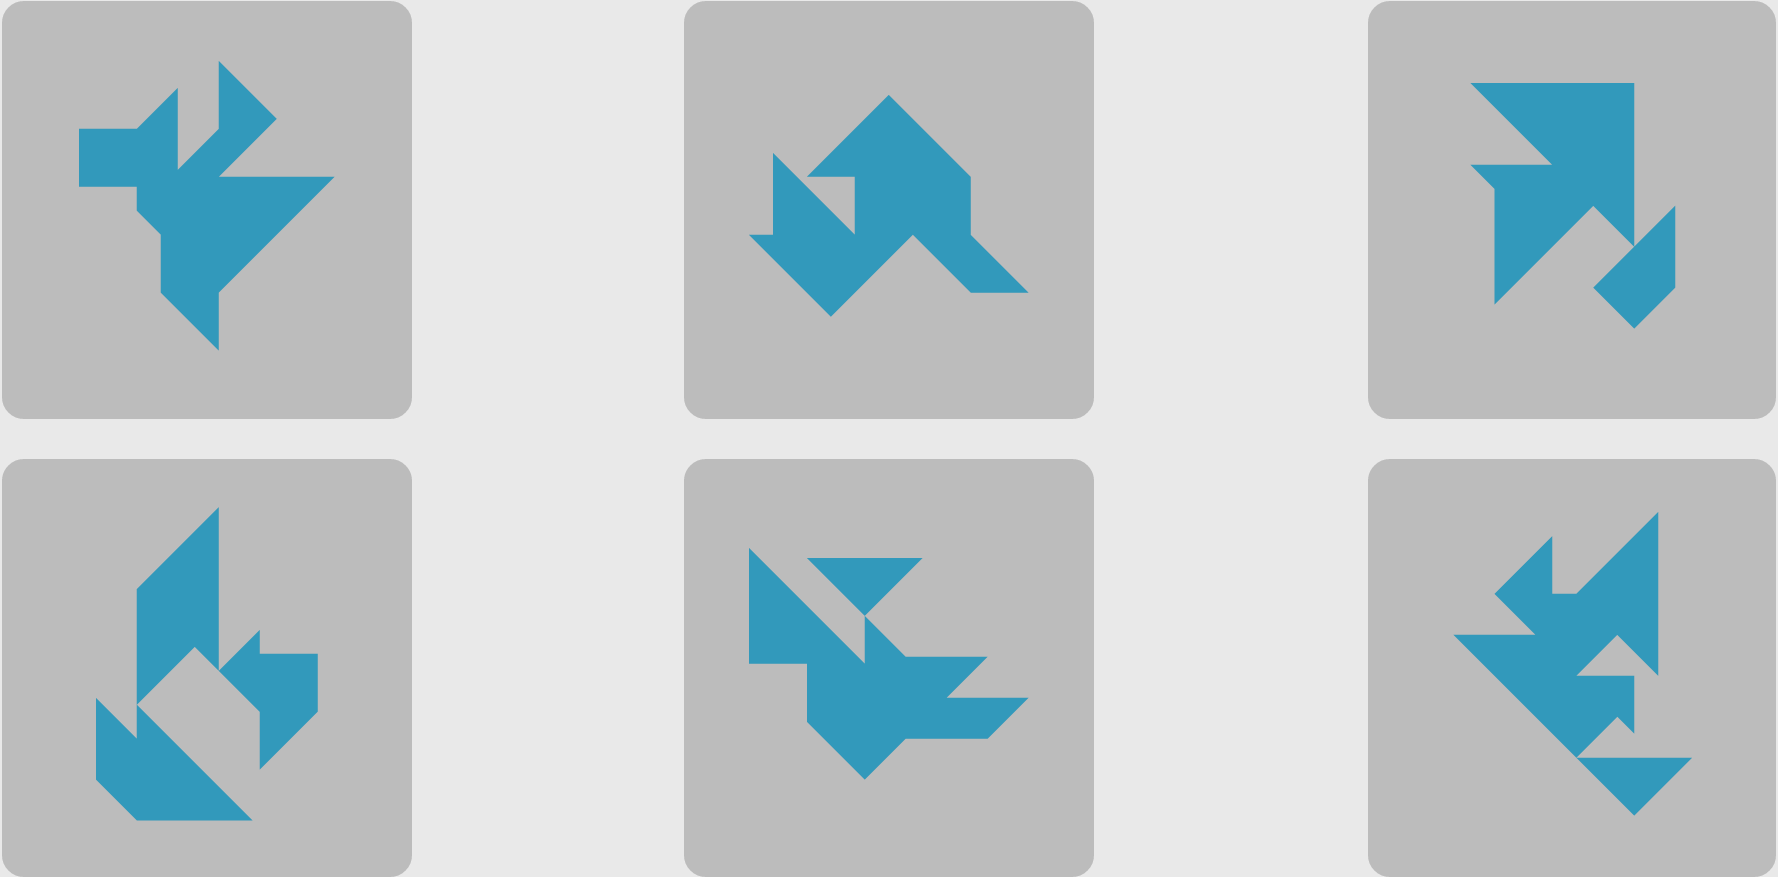
\includegraphics[width=0.45\textwidth]{figures/edgesLW.png}}
    \hfill
  \subfloat[Edge-matching approach with lower edge-matching weight]{\label{figur:6}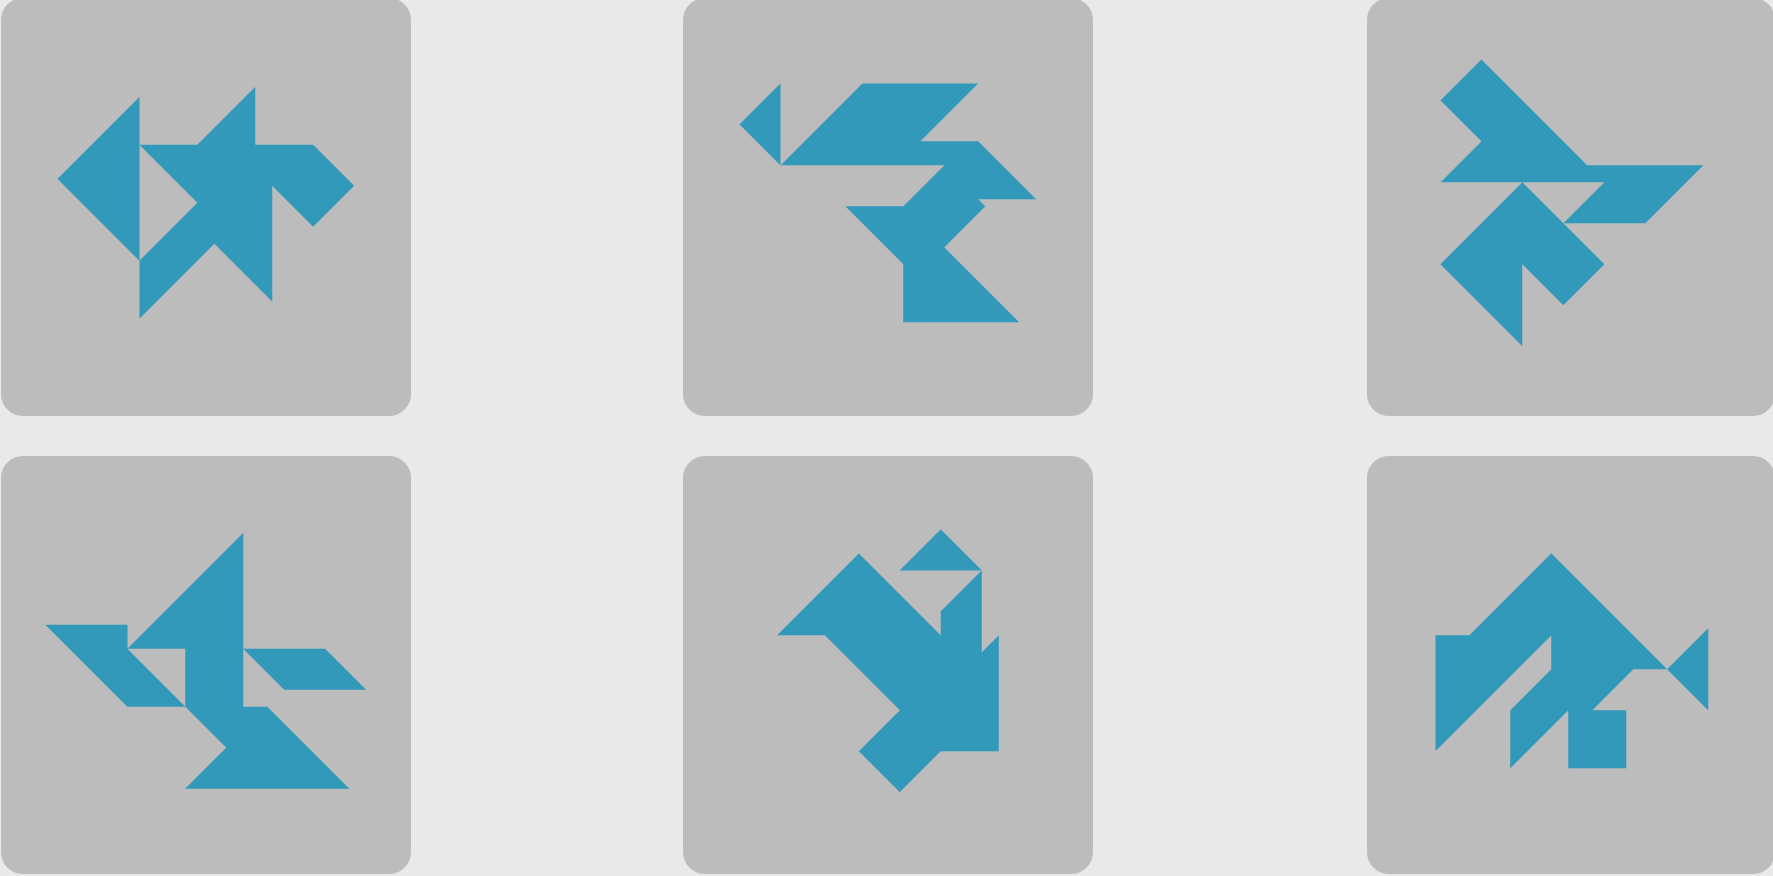
\includegraphics[width=0.45\textwidth]{figures/edgesSW}}
\caption{Results of generating six tangrams with different algorithms and different parameter settings}
\label{eval1}
\end{figure}

\section{Interestingness Measures}

The properties presented in section \ref{interesting}. Figure \ref{eval2} shows a few example for such measures. As expected, ranking according to both a high convex hull percentage and a low number of outline vertices leads to quite compact tangrams which are possibly harder to solve than tangrams where the tan pattern is more evident. Combining these two measures, leads to figures that are a bit less compact \begin{figure}[htp]
  \centering
  \subfloat[Ranking based on a high convex hull percentage]{\label{figur:1}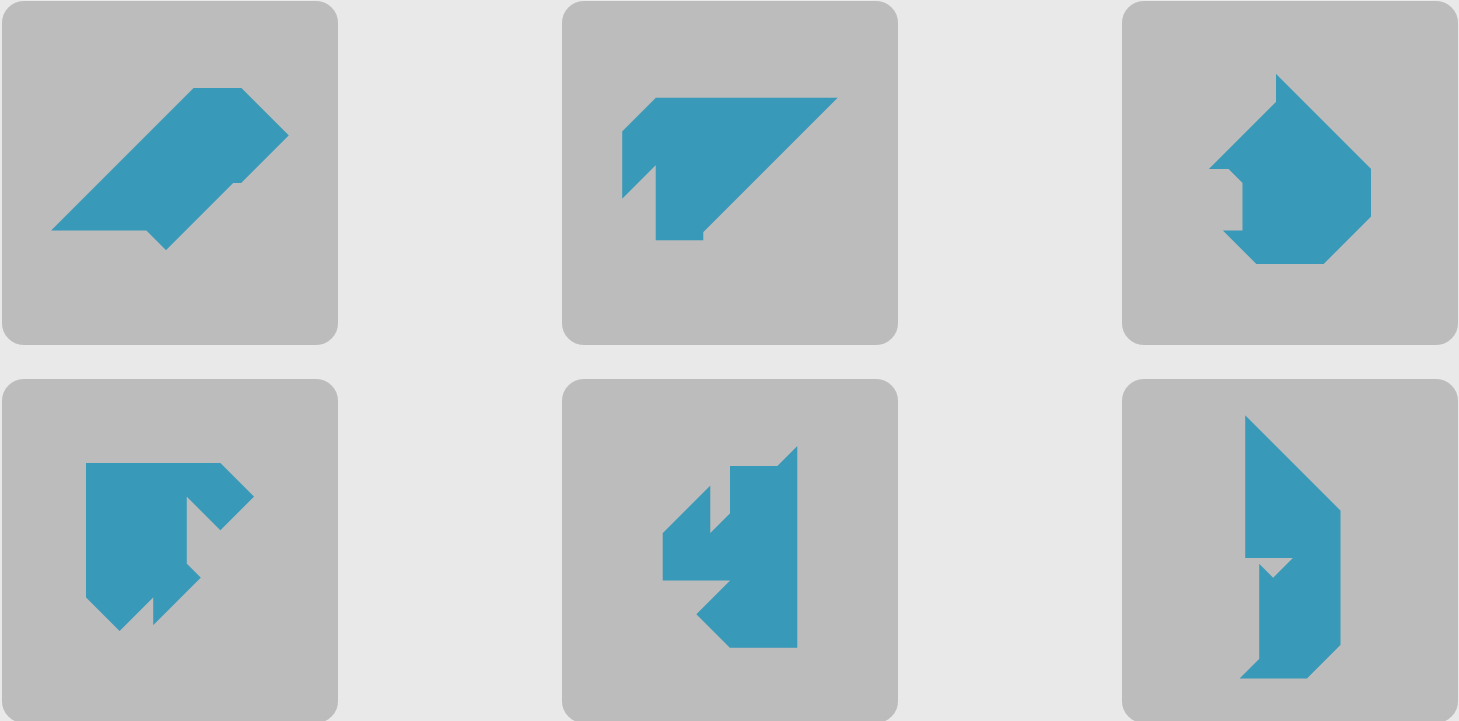
\includegraphics[width=0.45\textwidth]{figures/convexitypercentage.png}}
  \hfill
  \subfloat[Ranking based on a low number of outline vertices]{\label{figur:2}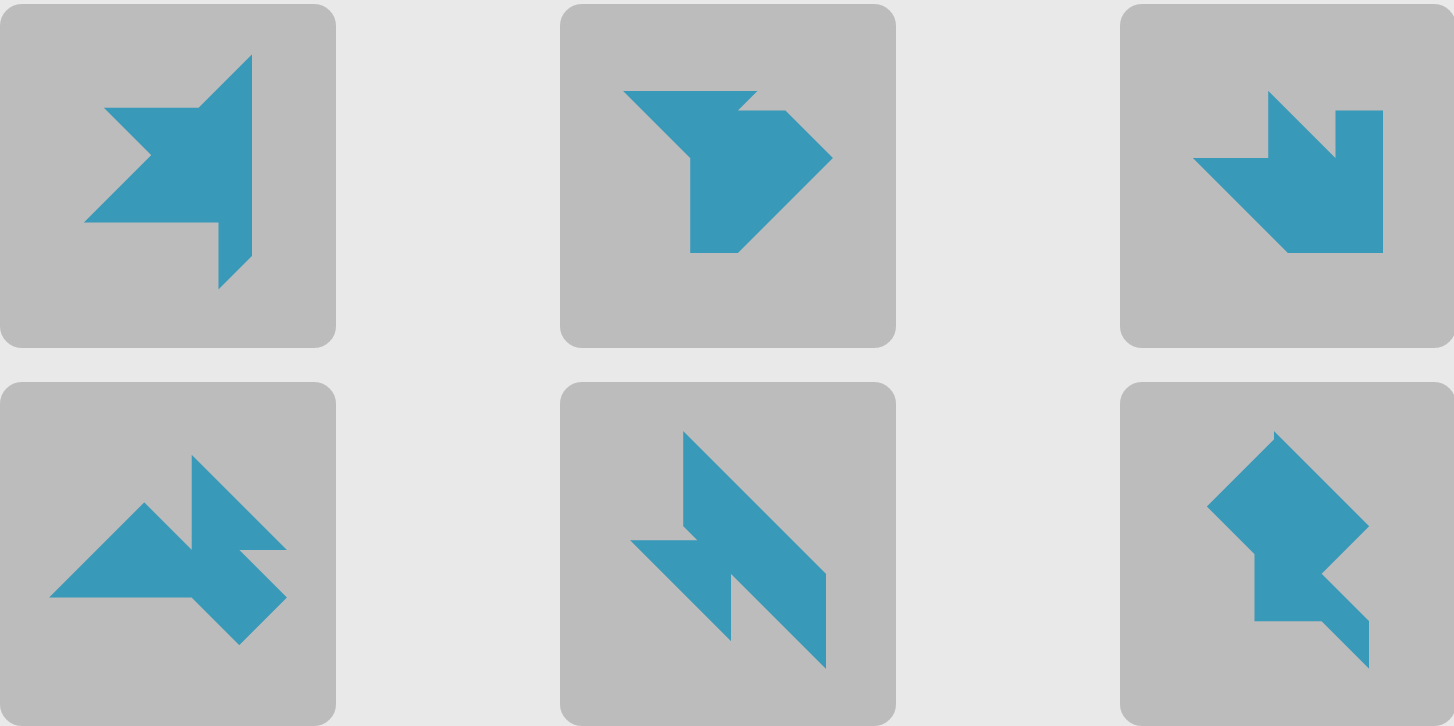
\includegraphics[width=0.45\textwidth]{figures/outlineVertices.png}}
  \\
  \subfloat[Ranking based on a high convex hull percentage and a low number of outline vertices]{\label{figur:3}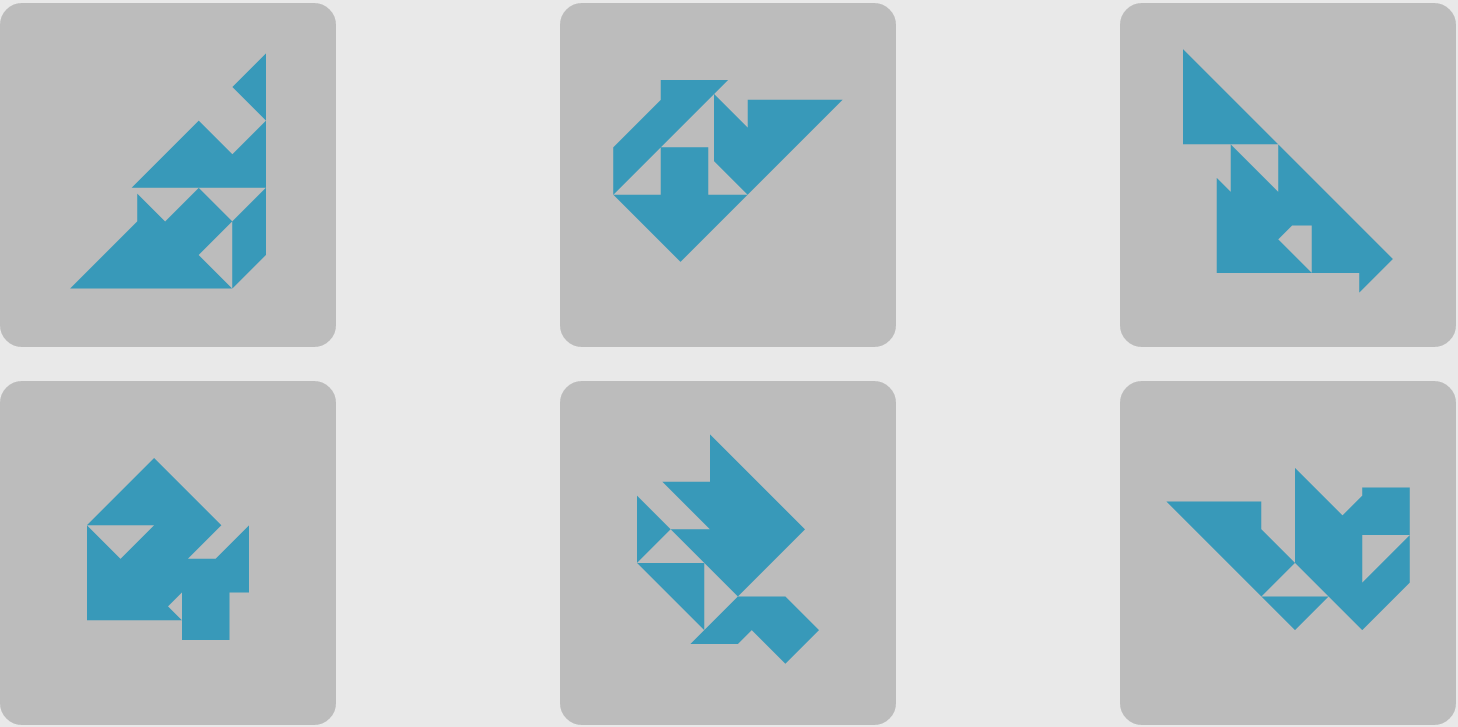
\includegraphics[width=0.45\textwidth]{figures/comine.png}}
    \hfill
  \subfloat[Ranking based on a high convex hull percentage and a low number of outer outline vertices]{\label{figur:4}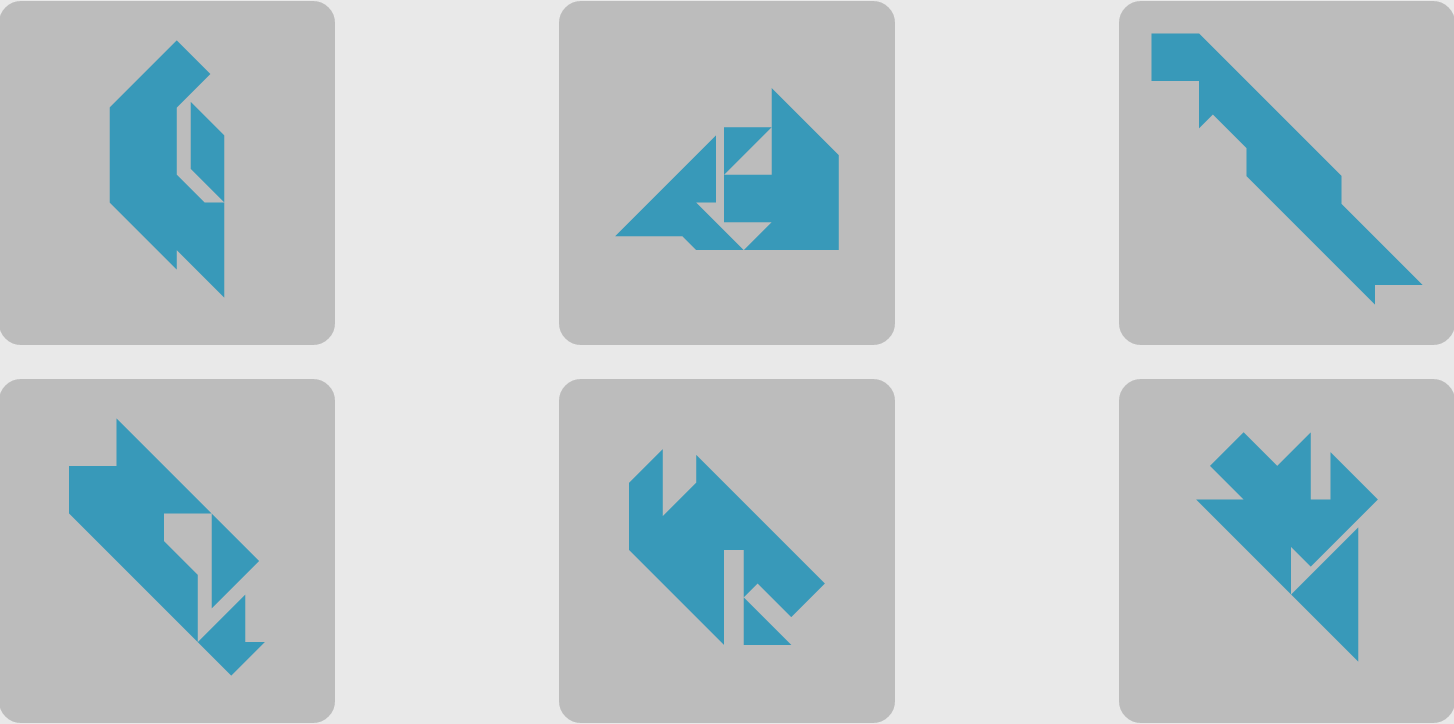
\includegraphics[width=0.45\textwidth]{figures/combineOuter.png}}
  \\
  \subfloat[Ranking based on a high number of matched vertices]{\label{figur:5}
\includegraphics[width=0.45\textwidth]{figures/matchedV.png}}
    \hfill
  \subfloat[Ranking based on a short shortest edge]{\label{figur:6}
\includegraphics[width=0.45\textwidth]{figures/shortestEdge.png}}
\caption{Results of generating 10.000 tangrams and ranking them according to different interestingness measures}
\label{eval2}
\end{figure}. Another promising measure is based on ranking according to a high number of matched vertices which should favour shape where at least part of tangram features an underlying star-like structure, as many pieces surround one point. Subjectively, the tangrams sorted to the top with this measure come closest to representing real world objects. 

\subsection{User study}

In addition to the interface described in the beginning of chapter \ref{chapter:design} an evaluation interface has been created in order to conduct a first user study. After generating tangrams, the users were presented with six tangrams for ten times and instructed to each time choose the shape that they found most interesting among the six. The presented tangrams were chosen randomly and without any sorting. In four cases, a part of the generated tangrams was filtered using certain properties and a random subset of the filtered tangrams was shown. Additionally, the first six shapes were not part of the set of randomly generated tangrams, but the same for all users. Figure \ref{result} shows a statistical analysis for the choice of the 53 participants in the case of the first six shapes. The shapes are ordered according to their rank determined by the percentage of users that chose the respective tangram as the most interesting one. The diagram also displays which rank among the six, the most expressive properties for the chosen tangrams would have reached if the tangrams were ordered according to the respective measure. Surprisingly, ranking according to a high number of (outer) outline vertices comes closest to the actual ranking at least for the two shapes that have been chosen as the most interesting ones by the majority. This result can probably not be generalised however, as only a single choice has been analysed here. Additionally, users chose only one shape as the most interesting one, which provides no information on their notion of interestingness of the other shapes.

\begin{figure}
\centering
    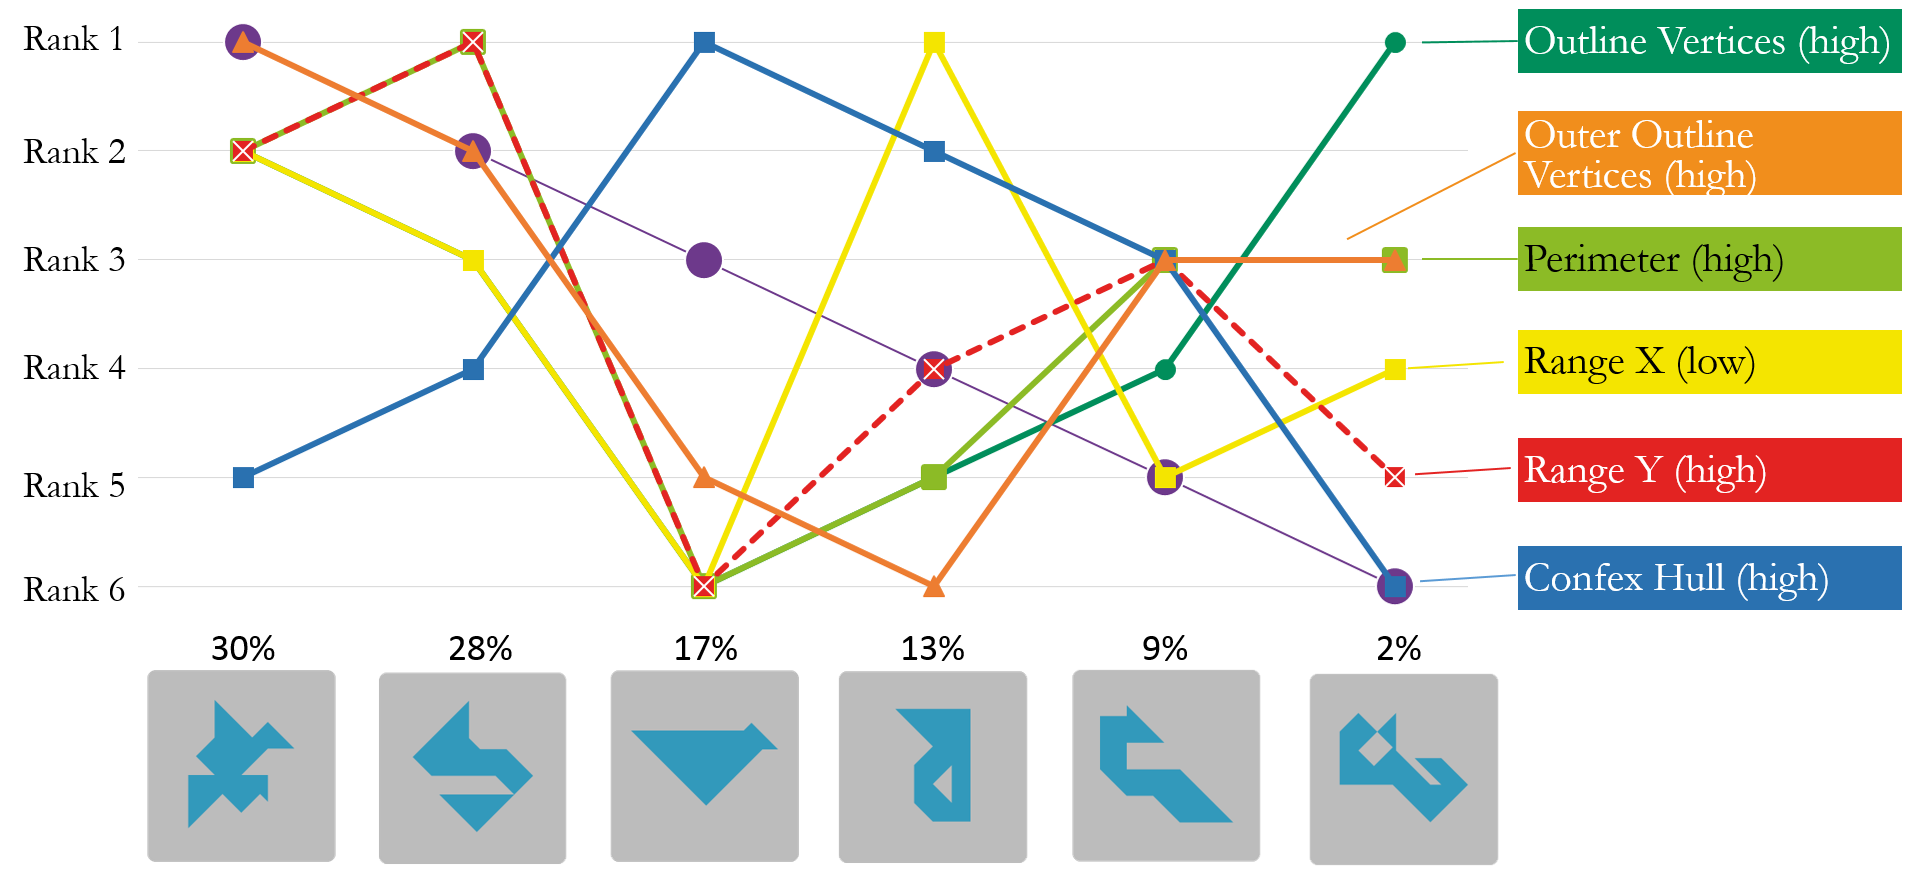
\includegraphics[width=0.95\textwidth]{figures/diagram.png}
  \caption{Result }  
  \label{result}
\end{figure}